\chapter{Resultados}

La figura \ref{fig:k} muestra el error cuadr\'atico de estimaci\'on de grupos en la poblaci\'on CHIBCHA para toda la muestra, sin haber eliminado ning\'un SNP. Este proceso de Cross-Validation muestra que en nuestra base de datos existe tres grupos, esto puede justificarse con la historia de conquista en M\'exico.\\

\begin{figure}[H]
  \centering
  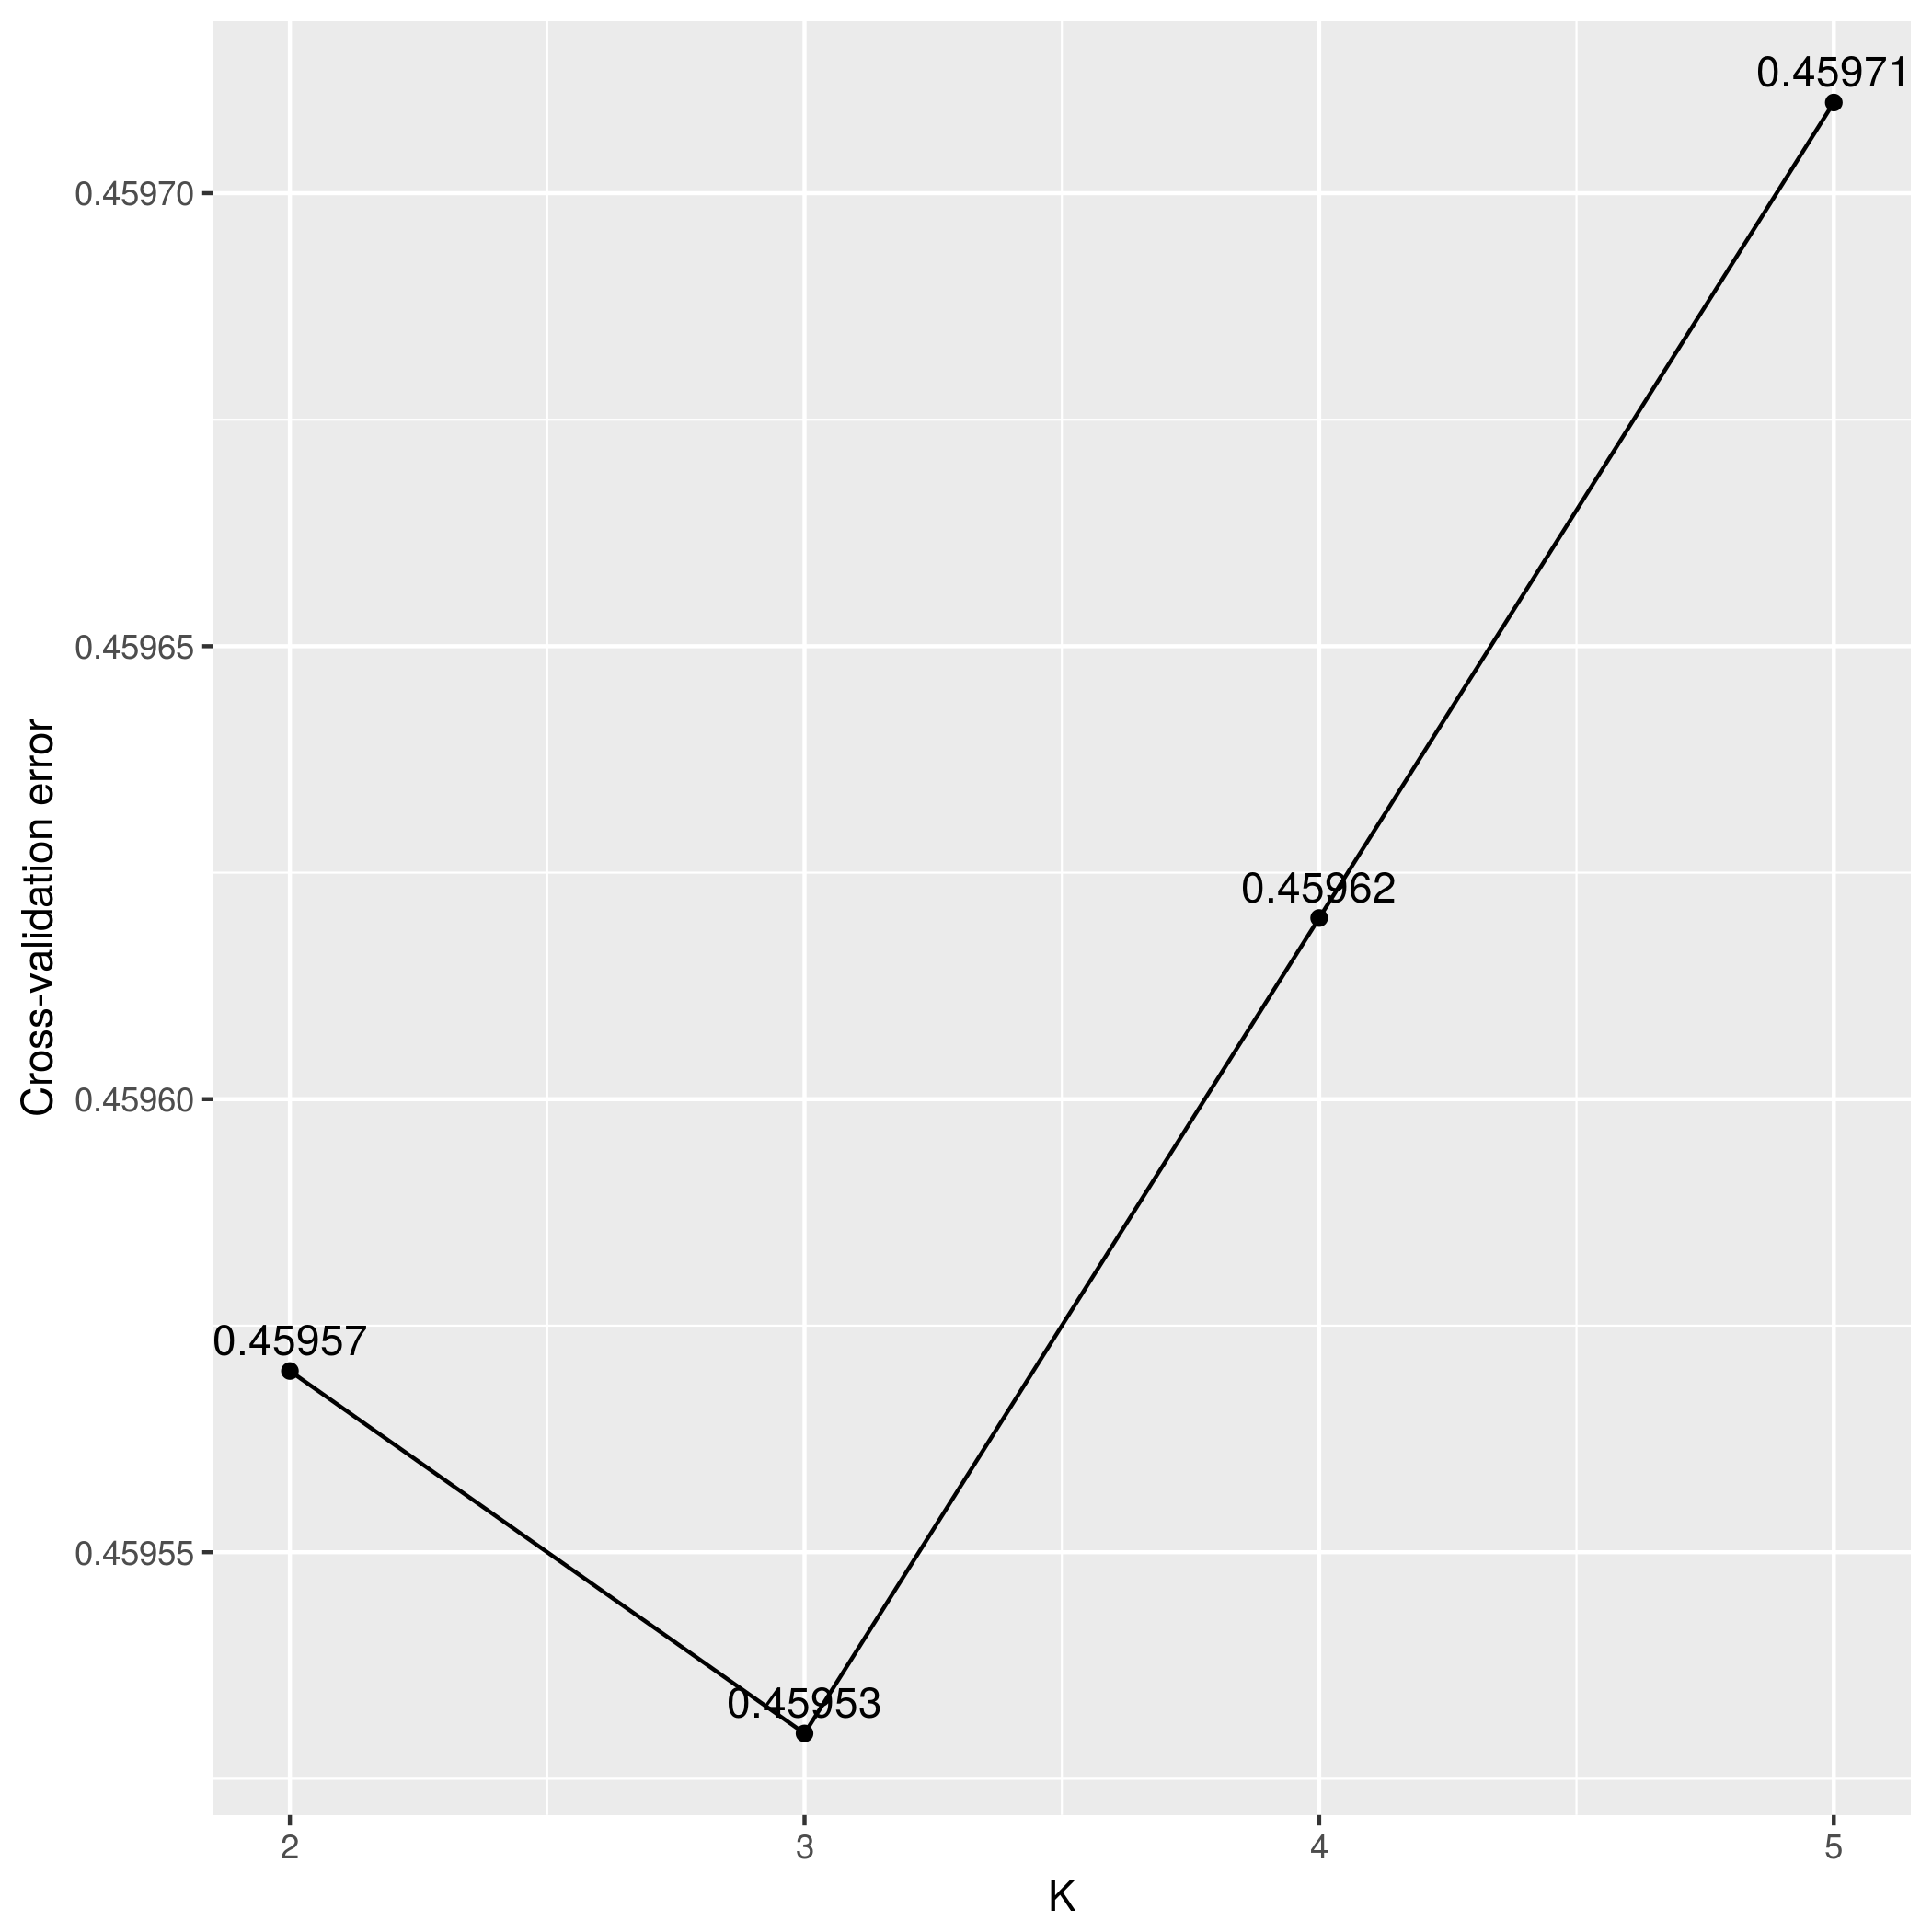
\includegraphics[scale = 0.5]{K5.png}
  \caption[Estimaci\'on de n\'umero de poblaciones]{Estimaci\'on de K, n\'umero de poblaciones posibles en la base de datos CHIBCHA.}
  \label{fig:k}
\end{figure}


\begin{table}[H]
  \centering
  \begin{tabular}{|l|l l|}
    \hline \hline
    & pob0& \\
    \hline
    pob0&&\\
    pob1&0.109&\\
    \hline \hline
  \end{tabular}
  \caption{Fst divergencia entre las poblaciones estimadas para K=2}
\end{table}

\begin{table}[H]
  \centering
  \begin{tabular}{|l| l l|}
    \hline \hline
    & pob0& pob1\\
    \hline
    pob1&0.017&\\
    pob2&0.121&0.082\\
    \hline \hline
  \end{tabular}
  \caption{Fst divergencia entre las poblaciones estimadas para K=3}
  \label{table:k3}
\end{table}

\begin{table}[H]
  \centering
  \begin{tabular}{|l| l l l|}
    \hline \hline
    & pob0& pob1&pob2\\
    \hline
    pob1&0.035& &\\
    pob2&0.089&0.061&\\
    pob3&0.119&0.078&0.015\\
    \hline \hline
  \end{tabular}
  \caption{Fst divergencia entre las poblaciones estimadas para K=4}
\end{table}



\begin{table}[H]
  \centering
  \begin{tabular}{|l| l l l l|}
    \hline \hline
    & pob0& pob1&pob2&pob3\\
    \hline
    pob1&0.067& & &\\
    pob2&0.050&0.055& &\\
    pob3&0.017&0.082&0.058&\\
    pob4&0.92&0.041&0.057&0.121\\
    \hline \hline
  \end{tabular}
  \caption{Fst divergencia entre las poblaciones estimadas para K=5}
\end{table}

Las tablas de divergencias nos muestran la separaci\'on entre las poblaciones estimadas. En este caso en particular se enfoca en la tabla \ref{table:k3} donde se observa que la poblaci\'on 2 y la poblaci\'on 0 tienen el valor de correlaci\'on m\'as alta, lo cual puede indicar que en estas poblaciones existen alelos iguales proviniente de una poblaci\'on ancestral.\\

Por otro lado, en la figura \ref{fig:an} podemos observar la derivaci\'on de las tres poblaciones utilizadas para este estudio (española, m\'exicana y africana). De manera similar podemos visualizar que la mayor\'ia de los individuos tienen poca frecuencia de la poblaci\'on africana, esto comprueba lo que se viene observando a trav\'es de la historia de la conquista en M\'exico.\\

\begin{figure}[H]
  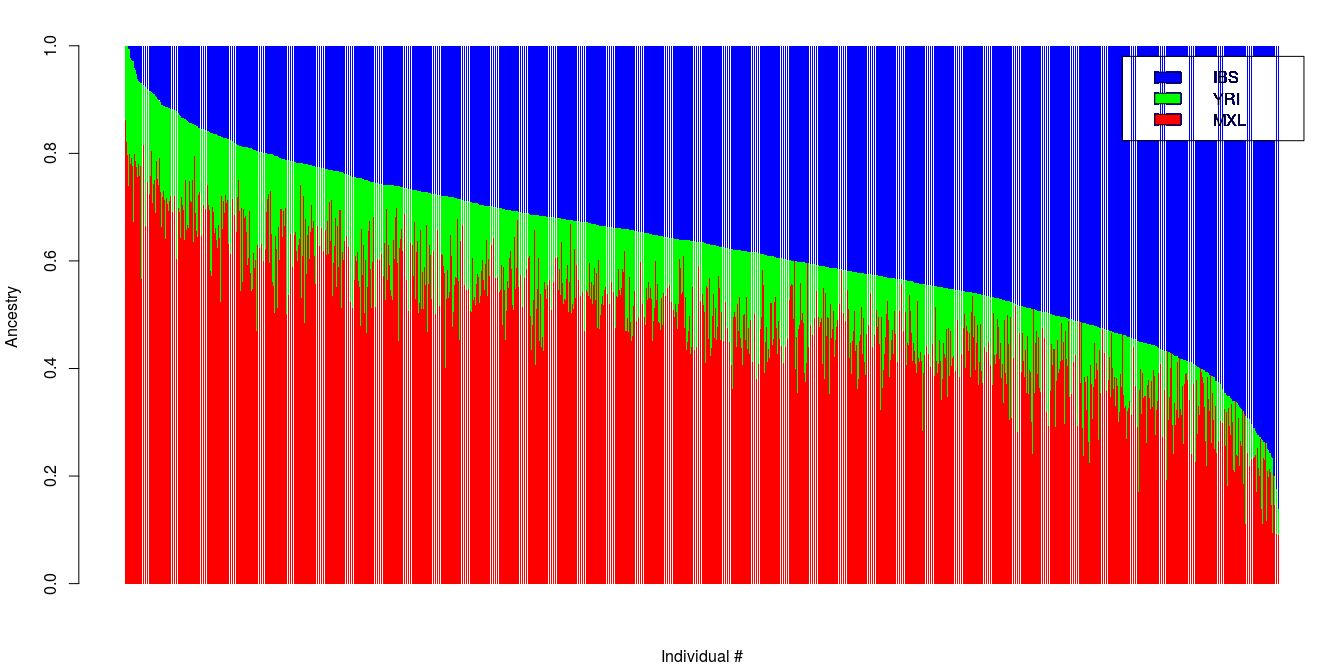
\includegraphics[scale=0.3]{Pro.png}
  \caption[Mapa de color para casos y controles]}{An\'alisis individual de ancestr\'ia total (casos y controles). Cada individuo es representado por una barra vertical en la gr\'afica.}
  \label{fig:an}
\end{figure}

\begin{figure}[H]
  \centering
  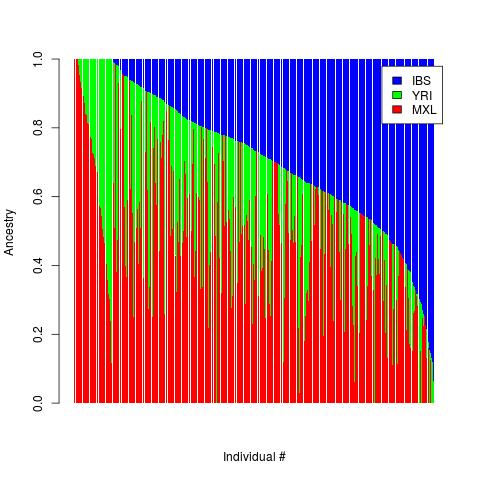
\includegraphics[scale=0.7]{rplot.jpg}
  \caption[Mapa de color para casos]{An\'alisis individual de ancestr\'ia para casos. Cada individuo es representado por una barra vertical en la gr\'afica.}
  \label{fig:ca}
\end{figure}

La figura \ref{fig:ca} tiene individuos con $100\%$ ancestralidad mexicana y casos de individuos sin ningún porcentaje de genes con ancestralidad mexicana. Adem\'as de mostrar una diferencia, con respecto al crecimiento del color verde (poblaci\'on africana), con la figura \ref{fig:an}. Esto puede deberse a que los casos provienen de entidades como Veracruz o Guerrero dado porcentaje de ancestrilidad altos de la poblaci\'on ancestral africana. De manera similar, dado que los individuos no muestran un distribuci\'on heterog\'enea de colores, puede inferirse que la relaci\'on con genes asociados al c\'ancer colorrectal estar\'a distribuido equitativamente en las tres poblaciones. 


\begin{figure}[H]
  \centering
  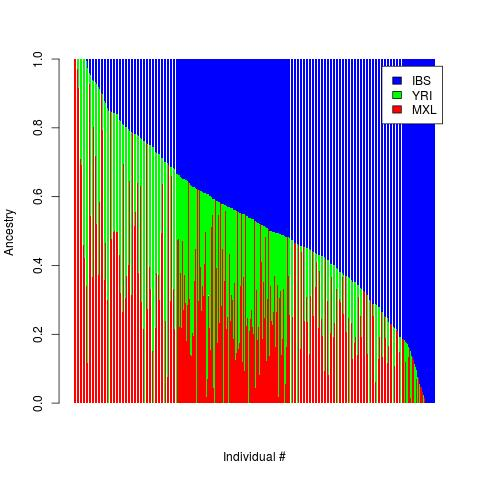
\includegraphics[scale=0.7]{r_malesplot.jpg}
  \caption[Mapa de color para casos masculino]{An\'alisis individual de ancestr\'ia para casos en g\'enero masculino. Cada individuo es representado por una barra vertical en la gr\'afica.}
  \label{fig:cam}
\end{figure}


\begin{figure}[H]
  \centering
  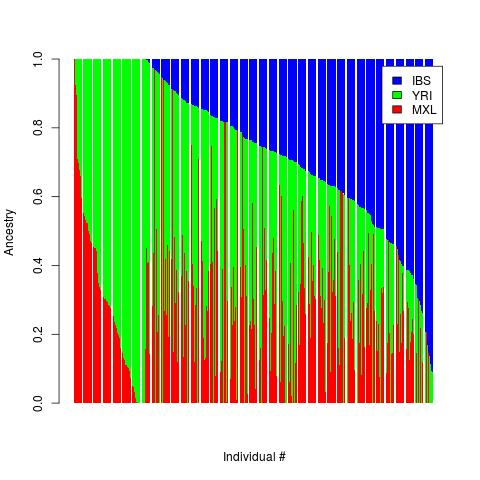
\includegraphics[scale=0.7]{r_femalesplot.jpg}
  \caption[Mapa de color para casos femenino]{An\'alisis individual de ancestr\'ia para casos en g\'enero femenino. Cada individuo es representado por una barra vertical en la gr\'afica.}
  \label{fig:caf}
\end{figure}


Con respecto a la posici\'on g\'enetica de los genes, y observando a cada indivudo en la gr\'afica \ref{fig:ca}, se obtuvo lo siguiente,\\

\begin{table}[H]
  \centering
  \begin{tabular}{|c|c|c|}
    \hline
    SNP & Locaci\'on& Poblaci\'on g\'enetica (\%)\\
    \hline
    rs74382455 & 1:84373659& Africana = 0.90\\
    rs2598121 & 7:37936286 & MXL = 0.96\\
    rs7311395 & 12:43574178 & Europea = 0.86\\
    rs7197593 & 16:55405713 & Europea = 0.97\\
    \hline
  \end{tabular}
\end{table}

De cuatro SNPs evaluados, dos de ellos tienen mayor porcentaje de poblaci\'on g\'enetica en españoles. Esto no implica que la poblaci\'on ancestral europea sea la de mayor correlaci\'on, si no que en estos cuatros SNPs tuvieron mayor relaci\'on. Puede ser que en los otros SNPs que no se mapearon pueda existir una ventaja de la misma poblaci\'on europea u otra de las dos.\\

Con respecto a las figuras \ref{fig:cam} y \ref{fig:caf} se puede observar que en el cuadro del g\'enero femenino existen mujeres con un porcentaje del 100 en genes con ascedencia \'africana, de manera similar, se puede observar que en el cuadro de hombres, hay individuos con porcentajes de 100 en ascedencia europea, esto siendo muy marcado en los distintos cuadros. 
